\documentclass{article}
\usepackage{graphicx}
\graphicspath{{images/}}

\title{Got It Diabetes Management:\\Mid-Point Design Document}
\date{2015-10-10}
\author{A Coursera Student}

\begin{document}
    \pagenumbering{gobble}
    \maketitle
    \newpage
    \pagenumbering{arabic}

    \section{User-Facing Components}

    In this section of the document you will see the app from a user's perspective, that is the screens and major features the user can use. The technical and implementation details will be described in the next section.

    \newpage

    \subsection{Authentication}

    A newly installed \emph{Diabetes Management} app should display the authentication screen to the user. Depending on whether the user has an existing account he/she needs to either log in or sign up (see the figure \ref{fig:screen_auth}).

    \begin{figure}[h]
        \centering
        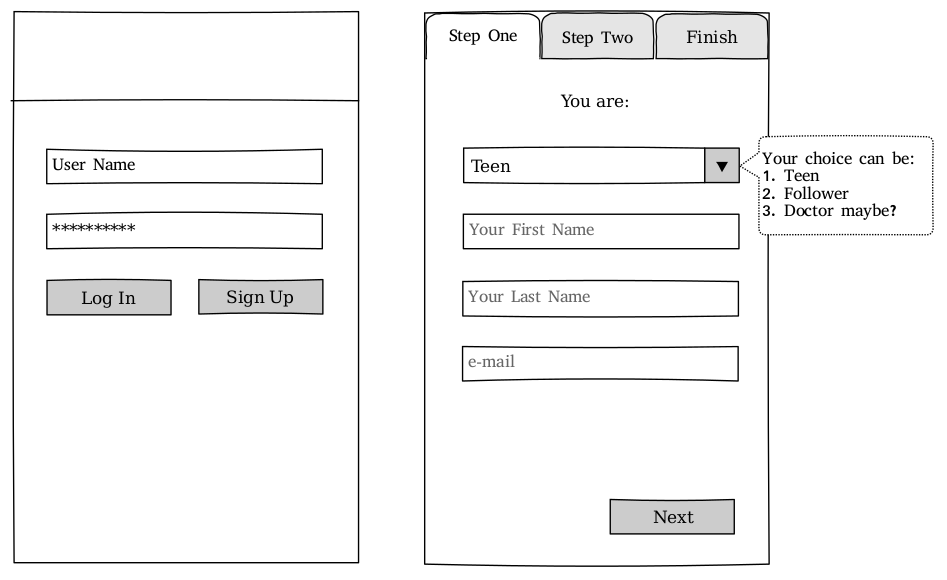
\includegraphics[width=\textwidth,height=\textheight,keepaspectratio]{auth.png}
        \caption{authentication screens}
        \label{fig:screen_auth}
    \end{figure}

    \begin{description}
        \item[Log In] \hfill \\
        The user needs to enter their user name (or e-mail) and password. After hitting on the Log In button the app will display the Check-In screen (see the figure \ref{fig:screen_checkin}).
        \item[Sign Up] \hfill \\
            The registration process includes several steps, each of which gathers various user's information. Depending on the user type (teen or follower), the information gathered might differ. The teen account will at least include a first name, a last name, a date of birth, and a medical record number. A followers account will probably only include a first and a last name.\footnote{Functional Description and App Requirement \#1: The Teen is the primary user of the mobile app and is represented in the app by a unit of data containing the core set of identifying information about a diabetic adolescent, including (but not necessarily limited to) a first name, a last name, a date of birth, and a medical record number.}
        \item[Log Out] \hfill \\
        As you can see in the figure \ref{fig:screen_main}, the user can also log out if, for example, another person needs to use the app under their own account.\footnote{Basic Project Requirement \#1: App supports multiple users via individual user accounts}
    \end{description}

    \newpage

    \subsection{Main Menu}

    To give the user ability to easily navigate between all the screens, the application uses a navigation drawer, which is called \emph{Main Menu}.\\Some menu items will indicated additional informations, for example, the number of unseen feedback, unread messages etc.

    \begin{figure}[h]
        \centering
        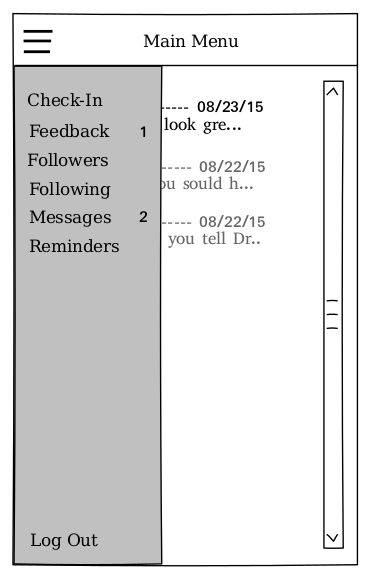
\includegraphics[width=0.5\textwidth,height=\textheight,keepaspectratio]{main.png}
        \caption{main menu}
        \label{fig:screen_main}
    \end{figure}


    This menu and the screens, which can be navigated to from the main menu, are only available to authenticated users.\footnote{Basic Project Requirement \#2: App contains at least one user facing function available only to authenticated users}

    \subsection{Check-In}


\end{document}
